% Date : 30/10/2022
% Version : 1
% Auteur : Écriture collective
% Relu : 
% Relecteur : 

% ------------------------------------------------------------ %
% ----------------------  Fiche A01  ------------------------- %
% Thème : Principe fondamental de la dynamique
% Classes : Toutes les classes de sup
% ------------------------------------------------------------ %



% ======================================================= % 
% ============== Gestion de la compilation ============== %
% ======================================================= % 
\ifdefined\mainIsLoaded\else
\RequirePackage{import}
\subimport{../../}{_preambule_CdE_PC}
\begin{document}
\fi
% ======================================================= % 
% ======================================================= % 

% ======================================================= % 
% ===================== Couleurs ======================== %
% ======================================================= % 

% -----------------------------------%
% La commande \couleurNBouCouleur prend deux paramètres :
% #1 est la couleur NB ; #2 est la couleur "en couleur"
\def\JRLblue{\couleurNBouCouleur{black}{blue!75}}
 \def\JRLblueC{\couleurNBouCouleur{lightgray!30}{blue!15}}
 \def\JRLblueF{\couleurNBouCouleur{gray}{blue!50}}
\def\JRLred{\couleurNBouCouleur{gray}{red!66}}
 \def\JRLcyan{\couleurNBouCouleur{gray}{cyan}}
 \def\JRLcyanclair{\couleurNBouCouleur{lightgray!30}{cyan!10}}
% ======================================================= % 





% ============================================================================ %
%                            FICHE D'ENTRAÎNEMENT                              %
% ============================================================================ %
% ======================= Métadonnées sur la fiche =========================== %
\titreFicheEntrainement		{Principe fondamental de la dynamique}
\grandTheme					{Mécanique}
\numeroFiche				{MCA02}
\uniqueID					{vLyJlwIhktp} % une chaîne de caractères (a-z, A-Z) aléatoire de 10 caractères.
\nombreColonnesReponses		{2} % 1, 2, 3, etc.
% ============================================================================ %

%%%%%%%%%%%%%%%%%%%%%%%%%%%%%%%%%%%%%%%%%%%%%%%%%%%%%%%%%%%%%%%%%%%%%%%%%%%%%%%%%%%%%%%%%%%%%%
\debutFicheEntrainement                                                                      %
%%%%%%%%%%%%%%%%%%%%%%%%%%%%%%%%%%%%%%%%%%%%%%%%%%%%%%%%%%%%%%%%%%%%%%%%%%%%%%%%%%%%%%%%%%%%%%




% --------------------------------------------------------------------- %
%                              Prérequis                                %
%                             (facultatif)                              %
% --------------------------------------------------------------------- %
% ================== Métadonnées sur le prérequis ===================== %
\avecPrerequis{Y} % Y ou N
% ===================================================================== %
\begin{prerequis}
	Projections. Coordonnées polaires. Équations différentielles simples.
\end{prerequis}
% --------------------------------------------------------------------- %







% •••••••••••••••••••••••••••••••••••••••••••••••••••••••••••••••••••••••••••• %
\sectionFicheEntrainement{Pour commencer}
% •••••••••••••••••••••••••••••••••••••••••••••••••••••••••••••••••••••••••••• %




% ********************************************************************* %
%                           ENTRAÎNEMENT                                % 
% ********************************************************************* %
% ================ Métadonnées sur l'entraînement ===================== %

\titreEntrainementFacultatif	{Une relation algébrique}
\hauteurLargeurCadreReponse		{1cm}{4.4cm}
\dureeResolutionFacultative		{1} % 1, 2, 3 ou 4
\typeEntrainement				{Newton} % Newton ou QCM ou AN ou vide (exercice "normal")
\basiqueEtTransversal			{Y}
\nombreColonnesQuestions		{1} % vide, 1, 2, 3, etc.
\avecPlusieursQuestions			{N} % Y ou N
\initialisationEntrainement
% ===================================================================== %


% =============================================================================== %
\debutEntrainement
% =============================================================================== %

	La vitesse $v$ (en régime permanent) d'un mobile vérifie l'équation
	\[
	m_1(v-v_1) + m_2(v-v_2) = p.\minusBigskip
	\]
	

% ^^^^^^^^^^^^^^^^^^^^^^^^^^^^^^^^^^^^^^ %
%               Question                 %
% ^^^^^^^^^^^^^^^^^^^^^^^^^^^^^^^^^^^^^^ %

\begin{enonce}
Donner l'expression de $v$ (en fonction de $m_1$, $m_2$, $v_1$, $v_2$ et $p$)
\end{enonce}

\reponse{$\frac{p+m_1v_1 + m_2v_2}{m_1+m_2}$}

%\begin{corrige}
%\end{corrige}

% ************************************** %

% =============================================================================== %
\finEntrainement
% =============================================================================== %

% ********************************************************************* %
%                           ENTRAÎNEMENT                                % 
% ********************************************************************* %
% ================ Métadonnées sur l'entraînement ===================== %

\titreEntrainementFacultatif	{Un système de deux équations}
\hauteurLargeurCadreReponse		{1cm}{4.4cm}
\dureeResolutionFacultative		{2} % 1, 2, 3 ou 4
\typeEntrainement				{Newton} % Newton ou QCM ou AN ou vide (exercice "normal")
\basiqueEtTransversal			{Y}
\nombreColonnesQuestions		{1} % vide, 1, 2, 3, etc.
\avecPlusieursQuestions			{Y} % Y ou N
\initialisationEntrainement
% ===================================================================== %


% =============================================================================== %
\debutEntrainement
% =============================================================================== %

Un problème de mécanique fait intervenir une force d'intensité $F$ et un angle  
$\alpha\in \left [0,\frac{\pi}{2} \right]$. En projetant la seconde loi de Newton sur deux axes, on aboutit au système d'équations suivant :
	\[
	\systeme[T,F]{T+F\sin\alpha=mR\omega^2, F\cos\alpha=mg.}\minusBigskip
	\]

% ^^^^^^^^^^^^^^^^^^^^^^^^^^^^^^^^^^^^^^ %
%               Question                 %
% ^^^^^^^^^^^^^^^^^^^^^^^^^^^^^^^^^^^^^^ %

\begin{enonce}
Déterminer $F$ en fonction des données $T$, $m$, $R$, $\omega$ et $g$.
\end{enonce}

\reponse{$\sqrt{\left(mR\omega^2-T\right)^2+(mg)^2}$}

\begin{corrige}
	Pour obtenir $F$ il faut pouvoir éliminer $\alpha$. L'astuce consiste à utiliser l'identité
	\[\sin^2\alpha+\cos^2\alpha=1.\]
	On a $\systeme[T,F]{F\sin\alpha=mR\omega^2-T,F\cos\alpha=mg}$ soit $F^2(\sin^2\alpha+\cos^2\alpha)=F^2=\left(mR\omega^2-T\right)^2+(mg)^2$. Finalement, l'intensité d'une force étant positive, on trouve $F=\sqrt{\left(mR\omega^2-T\right)^2+(mg)^2}$.
\end{corrige}

% ************************************** %

% ^^^^^^^^^^^^^^^^^^^^^^^^^^^^^^^^^^^^^^ %
%               Question                 %
% ^^^^^^^^^^^^^^^^^^^^^^^^^^^^^^^^^^^^^^ %

\begin{enonce}
Déterminer $\alpha$ en fonction des données $T$, $m$, $R$, $\omega$ et $g$.
\end{enonce}

\reponse{$\arctan{\left(\frac{mR\omega^2-T}{mg}\right)}$}

\begin{corrige}
	Quand on écrit le système sous la forme $\systeme[T,F]{F\sin\alpha=mR\omega^2-T,F\cos\alpha=mg}$, on s'aperçoit qu'il suffit de faire le rapport des deux équations pour éliminer $F$. On obtient 
	\[
		\tan\alpha=\frac{mR\omega^2-T}{mg}
		\quad\text{d'où}\quad
		\alpha=\arctan{\left(\frac{mR\omega^2-T}{mg}\right)}.
	\]
\end{corrige}

% ************************************** %

% =============================================================================== %
\finEntrainement
% =============================================================================== %



%
%
%% ********************************************************************* %
%%                           ENTRAÎNEMENT                                % 
%% ********************************************************************* %
%% ================ Métadonnées sur l'entraînement ===================== %
%\titreEntrainementFacultatif	{Analyse dimensionnelle}
%\hauteurLargeurCadreReponse		{7mm}{2cm}
%\dureeResolutionFacultative		{1} % 1, 2, 3 ou 4
%\typeEntrainement				{Newton} % Newton ou QCM ou AN ou vide (exercice "normal")
%\nombreColonnesQuestions		{1} % vide, 1, 2, 3, etc.
%\avecPlusieursQuestions			{Y} % Y ou N
%\initialisationEntrainement
%% ===================================================================== %
%
%
%% =============================================================================== %
%\debutEntrainement
%% =============================================================================== %
%
%
%% ^^^^^^^^^^^^^^^^^^^^^^^^^^^^^^^^^^^^^^ %
%%               Question                 %
%% ^^^^^^^^^^^^^^^^^^^^^^^^^^^^^^^^^^^^^^ %
%\begin{enonce}
%	Quelle est la dimension de la quantité de mouvement ?
%\end{enonce}
%
%\reponse{$\mathrm{MLT^{-1}}$}
%
%\begin{corrige}
%En effet, si on note $p$ la quantité de mouvement, $m$ la masse et $v$ la vitesse, on a $[p]=[mv]$, $[v]=\mathrm{LT^{-1}}$ et $[m]=\mathrm{M}$.
%\end{corrige}
%% ************************************** %
%
%
%% ^^^^^^^^^^^^^^^^^^^^^^^^^^^^^^^^^^^^^^ %
%%               Question                 %
%% ^^^^^^^^^^^^^^^^^^^^^^^^^^^^^^^^^^^^^^ %
%\begin{enonce}
%La constante de gravitation universelle vaut $\np[m^3.kg^{-1}.s^{-2}]{6,67e-11}$. \\
%Quelle est la dimension de la force gravitationnelle (et donc des autres forces) ?
%\end{enonce}
%
%\reponse{$\mathrm{MLT^{-2}}$}
%
%\begin{corrige}
%En vertu de la loi de gravitation universelle $F_\text{g}=\frac{Gm_1m_2}{r^2}$, d'où
%\[
%[F]=[G] \times \mathrm{M^2 L^{-2}} = \mathrm{L^3 M^{-1} T^{-2}}\times\mathrm{L^{-2}}=\mathrm{MLT^{-2}}
%\]
%\end{corrige}
%% ************************************** %
%
%% =============================================================================== %
%\finEntrainement
%% =============================================================================== %
%





% ********************************************************************* %
%                           ENTRAÎNEMENT                                % 
% ********************************************************************* %
% ================ Métadonnées sur l'entraînement ===================== %
\titreEntrainementFacultatif	{Quelques équations différentielles}
\hauteurLargeurCadreReponse		{10mm}{7cm}
\dureeResolutionFacultative		{2} % 1, 2, 3 ou 4
\typeEntrainement				{Newton} % Newton ou QCM ou AN ou vide (exercice "normal")
\basiqueEtTransversal			{Y}
\nombreColonnesQuestions		{1} % vide, 1, 2, 3, etc.
\avecPlusieursQuestions			{Y} % Y ou N
\initialisationEntrainement
% ===================================================================== %

Résoudre les équations différentielles suivantes, sachant que $v=0$ à $t=t_0$, et que les paramètres $a_0$ et $k$ sont des constantes.

% =============================================================================== %
\debutEntrainement
% =============================================================================== %


% ^^^^^^^^^^^^^^^^^^^^^^^^^^^^^^^^^^^^^^ %
%               Question                 %
% ^^^^^^^^^^^^^^^^^^^^^^^^^^^^^^^^^^^^^^ %
\begin{enonce}
	$\diff{v}{t} =  a_0$
\end{enonce}

\reponse{$a_0(t-t_0)$}

\begin{corrige}
La solution générale s'écrit $v(t)=a_0t+C_1$ où $C_1$ est une constante d'intégration que l'on détermine à l'aide de la condition $v(t_0)=0$. Cette condition donne $C_1=-a_0t_0$ d'où la solution $v(t)=a_0(t-t_0)$.
\end{corrige}
% ************************************** %

% ^^^^^^^^^^^^^^^^^^^^^^^^^^^^^^^^^^^^^^ %
%               Question                 %
% ^^^^^^^^^^^^^^^^^^^^^^^^^^^^^^^^^^^^^^ %
\begin{enonce}
	$\diff{v}{t} = -kv$
\end{enonce}

\reponse{$0$}

\begin{corrige}
La solution générale s'écrit $v(t) = A\eEuler^{-kt}$. La condition initiale $v(t_0)=0$ implique $A=0$ puisque $\eEuler^{-kt}>0$ pour tout $t$. Ainsi la solution est $v(t)=0$.
\end{corrige}
% ************************************** %

% ^^^^^^^^^^^^^^^^^^^^^^^^^^^^^^^^^^^^^^ %
%               Question                 %
% ^^^^^^^^^^^^^^^^^^^^^^^^^^^^^^^^^^^^^^ %
\begin{enonce}
	$\diff{v}{t} =  -kv+a_0$
\end{enonce}

\reponse{$\frac{a_0}{k}\left[1-\eEuler^{-k(t-t_0)}\right]$}

\begin{corrige}
La solution de l'équation homogène est $v(t) = A\eEuler^{-kt}$. Une solution particulière (constante) est $v = \frac{a_0}{k}$. Les solutions sont  $v(t) = A\eEuler^{-kt}+\frac{a_0}{k}$. La condition initiale $v(t_0)=0$ donne $A=-\frac{a_0}{k}\eEuler^{kt_0}$. Il en découle la solution générale : $v(t) = \frac{a_0}{k}\left[1-\eEuler^{-k(t-t_0)}\right]$.
\end{corrige}
% ************************************** %

% =============================================================================== %
\finEntrainement
% =============================================================================== %










\newpage



% •••••••••••••••••••••••••••••••••••••••••••••••••••••••••••••••••••••••••••• %
\sectionFicheEntrainement{Décomposition de vecteurs}
% •••••••••••••••••••••••••••••••••••••••••••••••••••••••••••••••••••••••••••• %




% ********************************************************************* %
%                           ENTRAÎNEMENT                                % 
% ********************************************************************* %
% ================ Métadonnées sur l'entraînement ===================== %
\titreEntrainementFacultatif	{Des projections}
\hauteurLargeurCadreReponse		{9mm}{5cm}
\dureeResolutionFacultative		{2} % 1, 2, 3 ou 4
\typeEntrainement				{Newton} % Newton ou QCM ou AN ou vide (exercice "normal")
\basiqueEtTransversal			{Y}
\nombreColonnesQuestions		{2} % vide, 1, 2, 3, etc.
\avecPlusieursQuestions			{Y} % Y ou N
\initialisationEntrainement
% ===================================================================== %

On considère les vecteurs suivants : 
\begin{center}
\subimport{_images/}{fiche_MCA02_figure_projection_1_CBD_v4.tex}
\end{center}

\vspace{-0.25cm}

Décomposer dans la base $(\vv{e_x}, \vv{e_y})$ les vecteurs :

% =============================================================================== %
\debutEntrainement
% =============================================================================== %



% ^^^^^^^^^^^^^^^^^^^^^^^^^^^^^^^^^^^^^^ %
%               Question                 %
% ^^^^^^^^^^^^^^^^^^^^^^^^^^^^^^^^^^^^^^ %
\begin{enonce}
	$\vv{a}$
\end{enonce}

\reponse{$a \cos(\alpha)\vv{e_x} + a \sin (\alpha) \vv{e_y}$}

\begin{corrige}


\pourcentageDeLaPartieAGauche   {0.55}
% -------------------- Partie à gauche -------------------- %
 \initialisationPartieGauche % 
% --------------------------------------------------------- %

La composante suivant $\vv{e_x}$ correspond au produit scalaire 
\[
\vv{a}\cdot \vv{e_x}=a\times 1\times \cos(\alpha).
\]
De même la composante suivant $\vv{e_y}$ est le produit scalaire  $\vv{a}\cdot \vv{e_y}=a\times 1\times \cos(\pi/2-\alpha)=a\sin(\alpha)$. On peut retrouver ces résultats géométriquement (\emph{cf}. ci-contre).

% --------------------------------------------------------- %
% -------------------- Partie à droite -------------------- %
 \initialisationPartieDroite %

\begin{center}
		%\subimport{_images/}{projection_1_cor_a_JRL_v1.tex}
		\def\longueurVecteurs{1.75}
\def\angle{45}
\begin{tikzpicture}
  \tikzstyle{fleche}=[->,>=stealth];
  \draw [fleche] (0,0) -- (\longueurVecteurs,0) node [above] {$\vv{e_x}$};
  \draw [fleche] (0,0) -- (0,\longueurVecteurs) node [right] {$\vv{e_y}$}; 
  \draw [fleche, very thick,\JRLblue] (0,0) -- (\angle:\longueurVecteurs) node [right] {$\vv{a}$};
  \draw [fleche] (\longueurVecteurs/2,0) arc (0:\angle:\longueurVecteurs/2) node [midway,right] {$\alpha$}; 
  \draw[fleche,thick]  (0,0)--(0:{\longueurVecteurs*cos(\angle)})node[below,midway]{$a\cos\alpha\vv{e_x}$};
   \draw[fleche,thick]  (0,0)--(90:{\longueurVecteurs*sin(\angle)})node[left,midway]{$a\sin\alpha\vv{e_y}$};
   \draw[dashed](90:{\longueurVecteurs*sin(\angle)})-|(0:{\longueurVecteurs*cos(\angle)});
\end{tikzpicture}
\end{center}
% --------------------------------------------------------- %
\finalisationDuPartageDePage %		
% --------------------------------------------------------- %
			
\end{corrige}

% ************************************** %



% ^^^^^^^^^^^^^^^^^^^^^^^^^^^^^^^^^^^^^^ %
%               Question                 %
% ^^^^^^^^^^^^^^^^^^^^^^^^^^^^^^^^^^^^^^ %
\begin{enonce}
	$\vv{b}$
\end{enonce}

\reponse{$b \sin(\alpha)\vv{e_x} + b \cos (\alpha) \vv{e_y}$}

 \begin{corrige}

\pourcentageDeLaPartieAGauche   {0.55}
% -------------------- Partie à gauche -------------------- %
 \initialisationPartieGauche % 

La composante suivant $\vv{e_x}$ vaut
\[
b_x=\vv{b}\cdot \vv{e_x}=b\cos(\pi/2-\alpha)=b\sin(\alpha).
\]
De même, la composante suivant $\vv{e_y}$ vaut 
\[
b_y=\vv{b}\cdot \vv{e_y}=b\cos(\alpha).
\]
% --------------------------------------------------------- %
% -------------------- Partie à droite ----------------- %
 \initialisationPartieDroite %
\begin{center}
		%\subimport{_images/}{projection_1_cor_b_JRL_v1.tex}
		\def\longueurVecteurs{1.75}
\def\angle{60}
\begin{tikzpicture}
  \tikzstyle{fleche}=[->,>=stealth];
  \draw [fleche] (0,0) -- (\longueurVecteurs,0) node [above] {$\vv{e_x}$};
  \draw [fleche] (0,0) -- (0,\longueurVecteurs) node [right] {$\vv{e_y}$}; 
  \draw [fleche, very thick,\JRLblue] (0,0) -- (\angle:\longueurVecteurs) node [right] {$\vv{b}$};
  \draw [fleche] (90:.5*\longueurVecteurs) arc (90:\angle:\longueurVecteurs/2) node [midway,above] {$\alpha$}; 
  \draw[fleche,thick]  (0,0)--(0:{\longueurVecteurs*cos(\angle)})node[below,midway]{$b\sin\alpha\vv{e_x}$};
   \draw[fleche,thick]  (0,0)--(90:{\longueurVecteurs*sin(\angle)})node[left,midway]{$b\cos\alpha\vv{e_y}$};
   \draw[dashed](90:{\longueurVecteurs*sin(\angle)})-|(0:{\longueurVecteurs*cos(\angle)});
\end{tikzpicture}

\end{center}
% --------------------------------------------------------- %
\finalisationDuPartageDePage %			

\end{corrige}

% ************************************** %



% ^^^^^^^^^^^^^^^^^^^^^^^^^^^^^^^^^^^^^^ %
%               Question                 %
% ^^^^^^^^^^^^^^^^^^^^^^^^^^^^^^^^^^^^^^ %
\begin{enonce}
	$\vv{c}$
\end{enonce}

\reponse{$c \cos(\alpha)\vv{e_x} - c \sin (\alpha) \vv{e_y}$}

\begin{corrigeNewpage}

\pourcentageDeLaPartieAGauche   {0.55}
% -------------------- Partie à gauche -------------------- %
 \initialisationPartieGauche % 


On a 
\[
c_x=\vv{c}\cdot \vv{e_x}=c\cos(\alpha)
\]
et 
\[
c_y=\vv{c}\cdot \vv{e_y}=c\cos(\pi/2+\alpha)=-c\sin(\alpha).
\]
On retrouve ces projections à l'aide de la construction ci-contre.
% --------------------------------------------------------- %
% -------------------- Partie à droite ----------------- %
 \initialisationPartieDroite %
\begin{center}
	%\subimport{_images/}{projection_1_cor_c_JRL_v1.tex}
	\def\longueurVecteurs{1.75}
\def\angle{-30}
\begin{tikzpicture}
  \tikzstyle{fleche}=[->,>=stealth];
  \draw [fleche] (0,0) -- (\longueurVecteurs,0) node [right] {$\vv{e_x}$};
  \draw [fleche] (0,0) -- (0,\longueurVecteurs) node [right] {$\vv{e_y}$}; 
  \draw [fleche, very thick,\JRLblue] (0,0) -- (\angle:\longueurVecteurs) node [right] {$\vv{c}$};
  \draw [fleche] (\longueurVecteurs/2,0) arc (0:\angle:\longueurVecteurs/2) node [midway,right] {$\alpha$}; 
  \draw[fleche,thick]  (0,0)--(0:{\longueurVecteurs*cos(\angle)})node[above,midway]{$c\cos\alpha\vv{e_x}$};
   \draw[fleche,thick]  (0,0)--(90:{\longueurVecteurs*sin(\angle)})node[left,midway]{$-c\sin\alpha\vv{e_y}$};
   \draw[dashed](90:{\longueurVecteurs*sin(\angle)})-|(0:{\longueurVecteurs*cos(\angle)});
\end{tikzpicture}

\end{center}
% --------------------------------------------------------- %
\finalisationDuPartageDePage %	

\end{corrigeNewpage}

% ************************************** %



% ^^^^^^^^^^^^^^^^^^^^^^^^^^^^^^^^^^^^^^ %
%               Question                 %
% ^^^^^^^^^^^^^^^^^^^^^^^^^^^^^^^^^^^^^^ %
\begin{enonce}
	$\vv{d}$
\end{enonce}

\reponse{$- d \sin(\alpha)\vv{e_x} + d \cos (\alpha) \vv{e_y}$}

\begin{corrige}

\pourcentageDeLaPartieAGauche   {0.55}
% -------------------- Partie à gauche -------------------- %
 \initialisationPartieGauche % 

On trouve 
\[
d_x=\vv{d}\cdot \vv{e_x}=d\cos(\pi/2+\alpha)=-d\sin(\alpha)
\]
et 
\[
d_y=\vv{d}\cdot \vv{e_y}=d\cos(\alpha).
\]
La construction ci-contre confirme ces projections.
% --------------------------------------------------------- %
% -------------------- Partie à droite ----------------- %
 \initialisationPartieDroite %
\begin{center}
	%\subimport{_images/}{projection_1_cor_d_JRL_v1.tex}
	\def\longueurVecteurs{1.75}
\def\angle{130}
\begin{tikzpicture}
  \tikzstyle{fleche}=[->,>=stealth];
  \draw [fleche] (0,0) -- (\longueurVecteurs,0) node [above] {$\vv{e_x}$};
  \draw [fleche] (0,0) -- (0,\longueurVecteurs) node [right] {$\vv{e_y}$}; 
  \draw [fleche, very thick,\JRLblue] (0,0) -- (\angle:\longueurVecteurs) node [above left] {$\vv{d}$};
  \draw [fleche] (90:\longueurVecteurs/2) arc (90:\angle:\longueurVecteurs/2) node [midway,above] {$\alpha$}; 
  \draw[fleche,thick]  (0,0)--(0:{\longueurVecteurs*cos(\angle)})node[below,midway]{$-d\sin\alpha\vv{e_x}$};
   \draw[fleche,thick]  (0,0)--(90:{\longueurVecteurs*sin(\angle)})node[right,midway]{$d\cos\alpha\vv{e_y}$};
   \draw[dashed](90:{\longueurVecteurs*sin(\angle)})-|(0:{\longueurVecteurs*cos(\angle)});
\end{tikzpicture}

\end{center}
% --------------------------------------------------------- %
\finalisationDuPartageDePage %	

\end{corrige}
% ************************************** %


% =============================================================================== %
\finEntrainement
% =============================================================================== %








% ********************************************************************* %
%                           ENTRAÎNEMENT                                % 
% ********************************************************************* %
% ================ Métadonnées sur l'entraînement ===================== %
\titreEntrainementFacultatif	{Sur un plan incliné}
\hauteurLargeurCadreReponse		{10mm}{5cm}
\dureeResolutionFacultative		{2} % 1, 2, 3 ou 4
\typeEntrainement				{Newton} % Newton ou QCM ou AN ou vide (exercice "normal")
\basiqueEtTransversal			{Y}
\nombreColonnesQuestions		{2} % vide, 1, 2, 3, etc.
\avecPlusieursQuestions			{Y} % Y ou N
\initialisationEntrainement
% ===================================================================== %



% mmmmmmmmmmmmmmmmmmmmmmmmmmmmmmmmmmmmmmmmmmmmmmmmmmmmmmmmm %
% 		  Insertion d'une image en regard d'un texte
% mmmmmmmmmmmmmmmmmmmmmmmmmmmmmmmmmmmmmmmmmmmmmmmmmmmmmmmmm %
% --------------------------------------------------------- %
\pourcentageDeLaPartieAGauche   {0.6}
% --------------------------------------------------------- %
%                                                           %
% -------------------- Partie à gauche -------------------- %
%                                                           %
                                \initialisationPartieGauche % 
%                                                           %
%                                                           %
On considère la situation représentée ci-contre.

Décomposer dans la base $(\vv{e_x}, \vv{e_y})$ les vecteurs suivants.
% --------------------------------------------------------- %
%                                                           %
% -------------------- Partie à droite -------------------- %
%                                                           %
                                \initialisationPartieDroite %
%                                                           %
%                                                           %
\begin{center}
\subimport{_images/}{fiche_MCA02_figure_projection_2_CBD_v5.tex}
\end{center}
% --------------------------------------------------------- %
                               \finalisationDuPartageDePage %					
% --------------------------------------------------------- %

\medskip


% =============================================================================== %
\debutEntrainement
% =============================================================================== %

% ^^^^^^^^^^^^^^^^^^^^^^^^^^^^^^^^^^^^^^ %
%               Question                 %
% ^^^^^^^^^^^^^^^^^^^^^^^^^^^^^^^^^^^^^^ %
\begin{enonce}
	$\vv{P}$
\end{enonce}

\reponse{$- P \sin(\alpha)\vv{e_x} - P \cos (\alpha) \vv{e_y}$}

\begin{corrige}
La composante suivant $\vv{e_x}$ du poids est $P_x=\vv{P}\cdot \vv{e_x}=P\cos(\alpha+\pi/2)=-P\sin(\alpha)$. De même, sa composante suivant $\vv{e_y}$ s'écrit $P_y=\vv{P}\cdot \vv{e_y}=P\cos(\alpha+\pi)=-P\cos(\alpha)$. Ainsi, le poids s'écrit 
\[
\vv{P} = - P \sin(\alpha)\vv{e_x} - P \cos (\alpha) \vv{e_y}.
\]
\end{corrige}
% ************************************** %

% ^^^^^^^^^^^^^^^^^^^^^^^^^^^^^^^^^^^^^^ %
%               Question                 %
% ^^^^^^^^^^^^^^^^^^^^^^^^^^^^^^^^^^^^^^ %
\begin{enonce}
	$\vv{N}$
\end{enonce}

\reponse{$N \vv{e_y}$}

\begin{corrige}
Le vecteur $\vv{N}$ est colinéaire au vecteur unitaire $\vv{e_y}$ et de même sens ; on a donc $\vv{N} = N \vv{e_y}$.
\end{corrige}
% ************************************** %

% =============================================================================== %
\finEntrainement
% =============================================================================== %









% ********************************************************************* %
%                           ENTRAÎNEMENT                                % 
% ********************************************************************* %
% ================ Métadonnées sur l'entraînement ===================== %
\titreEntrainementFacultatif	{Avec un pendule simple}
\hauteurLargeurCadreReponse		{9mm}{4.75cm}
\dureeResolutionFacultative		{2} % 1, 2, 3 ou 4
\typeEntrainement				{Newton} % Newton ou QCM ou AN ou vide (exercice "normal")
\basiqueEtTransversal			{Y}
\nombreColonnesQuestions		{2} % vide, 1, 2, 3, etc.
\avecPlusieursQuestions			{Y} % Y ou N
\initialisationEntrainement
% ===================================================================== %


On considère la situation 
\begin{center}
\subimport{_images/}{fiche_MCA02_pendule_simple_JRL_v3.tex}
\end{center}

Décomposer dans la base $(\vv{e_r}, \vv{e_\theta})$ les vecteurs suivants : 

% =============================================================================== %
\debutEntrainement
% =============================================================================== %

% ^^^^^^^^^^^^^^^^^^^^^^^^^^^^^^^^^^^^^^ %
%               Question                 %
% ^^^^^^^^^^^^^^^^^^^^^^^^^^^^^^^^^^^^^^ %
\begin{enonce}
	$\vv{P}$
\end{enonce}

\reponse{$ P \cos(\theta)\vv{e_r} - P \sin (\theta) \vv{e_\theta}$}

\begin{corrige}
La composante suivant $\vv{e_r}$ du poids est $P_r=\vv{P} \cdot \vv{e_r}=P\cos(\theta)$. De même, sa composante suivant $\vv{e_\theta}$ s'écrit $P_\theta=\vv{P}\cdot \vv{e_\theta}=P\cos(\alpha+\pi/2)=-P\sin(\theta)$. Ainsi, le poids s'écrit 
\[
\vv{P} = P \cos(\theta)\vv{e_r} - P \sin (\theta) \vv{e_\theta}.
\]
 \end{corrige}
% ************************************** %


% ^^^^^^^^^^^^^^^^^^^^^^^^^^^^^^^^^^^^^^ %
%               Question                 %
% ^^^^^^^^^^^^^^^^^^^^^^^^^^^^^^^^^^^^^^ %
\begin{enonce}
	$\vv{T}$
\end{enonce}

\reponse{$- T \vv{e_r}$}

\begin{corrige}
Le vecteur $\vv{T}$ est colinéaire au vecteur unitaire $\vv{e_r}$ et de sens opposé ; on a donc $\vv{T} =-T \vv{e_r}$.
\end{corrige}
% ************************************** %


% ^^^^^^^^^^^^^^^^^^^^^^^^^^^^^^^^^^^^^^ %
%               Question                 %
% ^^^^^^^^^^^^^^^^^^^^^^^^^^^^^^^^^^^^^^ %
\begin{enonce}
	$\vv{P}+\vv{T}$
\end{enonce}

\reponse{$(P \cos(\theta)-T)\vv{e_r} - P \sin (\theta) \vv{e_\theta}$}

%\begin{corrige}
%\end{corrige}
% ************************************** %


% =============================================================================== %
\finEntrainement
% =============================================================================== %



\newpage


% ********************************************************************* %
%                           ENTRAÎNEMENT                                % 
% ********************************************************************* %
% ================ Métadonnées sur l'entraînement ===================== %
\titreEntrainementFacultatif	{Avec un pendule simple (suite)}
\hauteurLargeurCadreReponse		{9mm}{4.75cm}
\dureeResolutionFacultative		{2} % 1, 2, 3 ou 4
\typeEntrainement				{Newton} % Newton ou QCM ou AN ou vide (exercice "normal")
\basiqueEtTransversal			{Y}
\nombreColonnesQuestions		{2} % vide, 1, 2, 3, etc.
\avecPlusieursQuestions			{Y} % Y ou N
\initialisationEntrainement
% ===================================================================== %

On se place dans la même situation que ci-dessus.
Décomposer dans la base $(\vv{e_x}, \vv{e_y})$ : 

\smallskip

% =============================================================================== %
\debutEntrainement
% =============================================================================== %

% ^^^^^^^^^^^^^^^^^^^^^^^^^^^^^^^^^^^^^^ %
%               Question                 %
% ^^^^^^^^^^^^^^^^^^^^^^^^^^^^^^^^^^^^^^ %
\begin{enonce}
	$\vv{P}$
\end{enonce}

\reponse{$P\vv{e_x}$}

\begin{corrige}
  Le poids $\vv{P}$ est colinéaire et de même sens que le vecteur unitaire $\vv{e_x}$ ; on a donc $\vv{P}=P\vv{e_x}$.
\end{corrige}
% ************************************** %


% ^^^^^^^^^^^^^^^^^^^^^^^^^^^^^^^^^^^^^^ %
%               Question                 %
% ^^^^^^^^^^^^^^^^^^^^^^^^^^^^^^^^^^^^^^ %
\begin{enonce}
	$\vv{T}$
\end{enonce}

\reponse{$-T\cos(\theta)\vv{e_x}-T\sin(\theta)\vv{e_y}$}

\begin{corrige}
La composante suivant $\vv{e_x}$ de la tension du fil $\vv{T}$ est $T_x=\vv{T}\cdot \vv{e_x}=T\cos(\pi-\theta)=-T\cos(\theta)$. 

De même, sa composante suivant $\vv{e_y}$ vaut $T_y=\vv{T}\cdot \vv{e_y}=T\cos(\pi/2+\theta)=-T\sin(\theta)$. Finalement, on trouve 
\[
\vv{T}=-T\cos(\theta)\vv{e_x}-T\sin(\theta)\vv{e_y}.
\]
\end{corrige}
% ************************************** %


% ^^^^^^^^^^^^^^^^^^^^^^^^^^^^^^^^^^^^^^ %
%               Question                 %
% ^^^^^^^^^^^^^^^^^^^^^^^^^^^^^^^^^^^^^^ %
\begin{enonce}
	$\vv{P}+\vv{T}$
\end{enonce}

\reponse{$(P-T\cos(\theta))\vv{e_x}-T\sin(\theta)\vv{e_y}$}

%\begin{corrige}
%\end{corrige}
% ************************************** %

% =============================================================================== %
\finEntrainement
% =============================================================================== %





% •••••••••••••••••••••••••••••••••••••••••••••••••••••••••••••••••••••••••••• %
\sectionFicheEntrainement{Entre accélération et position}
% •••••••••••••••••••••••••••••••••••••••••••••••••••••••••••••••••••••••••••• %




% ********************************************************************* %
%                           ENTRAÎNEMENT                                % 
% ********************************************************************* %
% ================ Métadonnées sur l'entraînement ===================== %
\titreEntrainementFacultatif	{Du vecteur position au vecteur accélération}
\hauteurLargeurCadreReponse		{2.5cm}{2cm}
\dureeResolutionFacultative		{1} % 1, 2, 3 ou 4
\typeEntrainement				{Reprise} % Newton ou QCM ou AN ou vide (exercice "normal")
\nombreColonnesQuestions		{3} % 1, 2, 3, etc.
\avecPlusieursQuestions			{Y} % Y ou N
\initialisationEntrainement
% ===================================================================== %

On considère un point $\ptM$ en mouvement dont les coordonnées cartésiennes dans la base $(\vv{e_x},\vv{e_y},\vv{e_z})$ sont, à chaque instant $x(t)=\frac12 a_0t^2 + x_0$, $y(t)=-v_0t$ et $z(t) = z_0$. 

Donner les expressions du vecteur:

% =============================================================================== %
\debutEntrainement
% =============================================================================== %

% ^^^^^^^^^^^^^^^^^^^^^^^^^^^^^^^^^^^^^^ %
%               Question                 %
% ^^^^^^^^^^^^^^^^^^^^^^^^^^^^^^^^^^^^^^ %
\begin{enonce}
	 position
\end{enonce}

\reponse{$\left(\frac12 a_0 t^2 + x_0\right)\vv{e_x} - v_0 t \vv{e_y} + z_0 \vv{e_z}$}

\begin{corrige}
	Le vecteur position est le vecteur $\vv{\text{OM}}=x\vv{e_x}+y\vv{e_y}+z\vv{e_z}$, d'où 
	\[
	\vv{\text{OM}} =\left(\frac12 a_0 t^2 + x_0\right)\vv{e_x} - v_0 t \vv{e_y} + z_0 \vv{e_z}.
	\]
\end{corrige}

% ************************************** %


% ^^^^^^^^^^^^^^^^^^^^^^^^^^^^^^^^^^^^^^ %
%               Question                 %
% ^^^^^^^^^^^^^^^^^^^^^^^^^^^^^^^^^^^^^^ %
\begin{enonce}
	  vitesse
\end{enonce}

\reponse{$a_0 t \vv{e_x} - v_0 \vv{e_y} $}

\begin{corrige}
Dans le système de coordonnées cartésiennes, le vecteur vitesse s'écrit 
\[
\vv{v}=\dot{x}\vv{e_x}+\dot{y}\vv{e_y}+\dot{z}\vv{e_z}=a_0 t \vv{e_x} - v_0 \vv{e_y}.
\]
\end{corrige}

% ************************************** %


% ^^^^^^^^^^^^^^^^^^^^^^^^^^^^^^^^^^^^^^ %
%               Question                 %
% ^^^^^^^^^^^^^^^^^^^^^^^^^^^^^^^^^^^^^^ %
\begin{enonce}
	 accélération
\end{enonce}

\reponse{$a_0 \vv{e_x}$}

\begin{corrige}
 Dans le système de coordonnées cartésiennes, le vecteur accélération s'exprime en fonction des dérivées secondes des coordonnées : $\vv{a} =\ddot{x}\vv{e_x}+\ddot{y}\vv{e_y}+\ddot{z}\vv{e_z}=a_0 \vv{e_x}$.
\end{corrige}

% ************************************** %
% =============================================================================== %
\finEntrainement
% =============================================================================== %






% ********************************************************************* %
%                           ENTRAÎNEMENT                                % 
% ********************************************************************* %
% ================ Métadonnées sur l'entraînement ===================== %
\titreEntrainementFacultatif	{Du vecteur accélération au vecteur position}
\hauteurLargeurCadreReponse		{2.5cm}{3cm}
\dureeResolutionFacultative		{1} % 1, 2, 3 ou 4
\typeEntrainement				{} % Newton ou QCM ou AN ou vide (exercice "normal")
\nombreColonnesQuestions		{2} % 1, 2, 3, etc.
\avecPlusieursQuestions			{Y} % Y ou N
\initialisationEntrainement
% ===================================================================== %

On considère un point $\ptM$ de masse $m$ en chute libre soumis à son poids $\vv{P}=mg\vv{e_z}$. Ce point $\ptM$ a été lancé avec une vitesse initiale $\vv{v_0} = v_0 \vv{e_x}$ et une position initiale $\ptM_0 \begin{pmatrix}x_0 \\ y_0 \\0\end{pmatrix}$.

Donner l'expression des vecteurs :


% =============================================================================== %
\debutEntrainement
% =============================================================================== %

% ^^^^^^^^^^^^^^^^^^^^^^^^^^^^^^^^^^^^^^ %
%               Question                 %
% ^^^^^^^^^^^^^^^^^^^^^^^^^^^^^^^^^^^^^^ %
\begin{enonce}
	 accélération
\end{enonce}

\reponse{$g \vv{e_z} $}

\begin{corrige}
  D'après le PFD, on a $mg\vv{e_z}=m\vv{a}$ d'où $\vv{a}=g \vv{e_z}$.
\end{corrige}

% ************************************** %


% ^^^^^^^^^^^^^^^^^^^^^^^^^^^^^^^^^^^^^^ %
%               Question                 %
% ^^^^^^^^^^^^^^^^^^^^^^^^^^^^^^^^^^^^^^ %
\begin{enonce}
	 vitesse
\end{enonce}

\reponse{$v_0 \vv{e_x} + g t \vv{e_z} $}

\begin{corrige}
  L'accélération s'écrit $\vv{a}=\dot{v}_x\vv{e_x}+\dot{v}_y\vv{e_y}+\dot{v}_z\vv{e_z}$. On en déduit 
  \[
  	\left\{
	\begin{array}{ccc}
  		\dot{v}_x&=&0\\
  		\dot{v}_y&=&0\\
  		\dot{v}_z&=&g\\
  	\end{array}
	\right.
	\quad\text{donc}\quad
  	\left\{
	\begin{array}{ccc}
  		v_x&=&C_1\\
  		v_y&=&C_2\\
  		v_z&=&gt+C_3.
  	\end{array}
	\right.
  \]
  Les conditions initiales imposent $C_1=v_0$, $C_2=0$ et $C_3=0$. Finalement, on trouve $\vv{v}=v_0 \vv{e_x} + g t \vv{e_z}$.
\end{corrige}

% ************************************** %


% ^^^^^^^^^^^^^^^^^^^^^^^^^^^^^^^^^^^^^^ %
%               Question                 %
% ^^^^^^^^^^^^^^^^^^^^^^^^^^^^^^^^^^^^^^ %
\begin{enonce}
	 position
\end{enonce}

\reponse{$(v_0 t + x_0) \vv{e_x} + y_0\vv{e_y}+ \frac12 gt^2 \vv{e_z}$}

\begin{corrige}
Le vecteur vitesse s'écrit $\vv{v}=\dot{x}\vv{e_x}+\dot{y}\vv{e_y}+\dot{z}\vv{e_z}$. 

Par identification avec l'expression obtenue précédemment, on a 
 \[
 \left\{
 \begin{array}{ccc}
 	\dot{x}&=&v_0\\
 	\dot{y}&=&0\\
 	\dot{z}&=&gt\\
 \end{array}
\right.
	\quad\text{donc}\quad
\left\{
\begin{array}{ccc}
	x&=&v_0t+C_4\\
	y&=&C_5\\
	z&=&\frac12 gt^2+C_6.
\end{array}
\right.
 \]
Les conditions initiales imposent $C_4=x_0$, $C_5=y_0$ et $C_6=0$. Finalement, on trouve
\[
\vv{\ptO\ptM}=(v_0 t + x_0) \vv{e_x} + y_0\vv{e_y}+ \frac12 gt^2 \vv{e_z}.
\]
\end{corrige}

% ************************************** %
% =============================================================================== %
\finEntrainement
% =============================================================================== %


\newpage


% •••••••••••••••••••••••••••••••••••••••••••••••••••••••••••••••••••••••••••• %
\sectionFicheEntrainement{Autour des coordonnées polaires}
% •••••••••••••••••••••••••••••••••••••••••••••••••••••••••••••••••••••••••••• %

\medskip

% mmmmmmmmmmmmmmmmmmmmmmmmmmmmmmmmmmmmmmmmmmmmmmmmmmmmmmmmm %
% 		  Insertion d'une image en regard d'un texte
% mmmmmmmmmmmmmmmmmmmmmmmmmmmmmmmmmmmmmmmmmmmmmmmmmmmmmmmmm %
% --------------------------------------------------------- %
\pourcentageDeLaPartieAGauche   {0.62}
% --------------------------------------------------------- %
%                                                           %
% -------------------- Partie à gauche -------------------- %
%                                                           %
                                \initialisationPartieGauche % 
%                                                           %
%                                                           %
Dans ce paragraphe, on considère un point M repéré par la distance~$r$ et l'angle~$\theta$ en coordonnées polaires. 
La distance $r$ et l'angle $\theta$ dépendent du temps $t$ : le point M est mobile.

\smallskip

On représente la situation par le schéma ci-contre.
% --------------------------------------------------------- %
%                                                           %
% -------------------- Partie à droite -------------------- %
%                                                           %
                                \initialisationPartieDroite %
%                                                           %
%                                                           %
\begin{center}
\subimport{_images/}{fiche_MCA02_coordonnes_polaires_JRL_v3.tex}
\end{center}
% --------------------------------------------------------- %
                               \finalisationDuPartageDePage %					
% --------------------------------------------------------- %


% ********************************************************************* %
%                           ENTRAÎNEMENT                                % 
% ********************************************************************* %
% ================ Métadonnées sur l'entraînement ===================== %
\titreEntrainementFacultatif	{Trois calculs fondamentaux}
\hauteurLargeurCadreReponse		{7mm}{4.5cm}
\dureeResolutionFacultative		{2} % 1, 2, 3 ou 4
\typeEntrainement				{Newton} % Newton ou QCM ou AN ou vide (exercice "normal")
\basiqueEtTransversal			{Y}
\nombreColonnesQuestions		{2} % 1, 2, 3, etc.
\avecPlusieursQuestions			{Y} % Y ou N
\initialisationEntrainement
% ===================================================================== %


Décomposer dans la base $(\vv{e_x}, \vv{e_y})$ les vecteurs : 

% =============================================================================== %
\debutEntrainement
% =============================================================================== %


% ^^^^^^^^^^^^^^^^^^^^^^^^^^^^^^^^^^^^^^ %
%               Question                 %
% ^^^^^^^^^^^^^^^^^^^^^^^^^^^^^^^^^^^^^^ %
\begin{enonce}
	$\vv{e_r}$
\end{enonce}

\reponse{$\cos(\theta) \vv{e_x} + \sin (\theta) \vv{e_y}$}

\begin{corrige}
On a  $\vv{e_r}\cdot\vv{e_x}=\cos(\theta)$ et  $\vv{e_r}\cdot\vv{e_y}=\cos(\pi/2-\theta)=\sin(\theta)$ d'où $\vv{e_r}=\cos(\theta) \vv{e_x} + \sin (\theta) \vv{e_y}$.
\end{corrige}
% ************************************** %


% ^^^^^^^^^^^^^^^^^^^^^^^^^^^^^^^^^^^^^^ %
%               Question                 %
% ^^^^^^^^^^^^^^^^^^^^^^^^^^^^^^^^^^^^^^ %
\begin{enonce}
	$\vv{e_\theta}$
\end{enonce}

\reponse{$- \sin(\theta) \vv{e_x} + \cos (\theta) \vv{e_y}$}

\begin{corrige}
On a  $\vv{e_\theta}\cdot\vv{e_x}=\cos(\pi/2+\theta)=-\sin(\theta)$ et  $\vv{e_\theta}\cdot\vv{e_y}=\cos(\theta)$ d'où $\vv{e_\theta}=- \sin(\theta) \vv{e_x} + \cos (\theta) \vv{e_y}$.
\end{corrige}
% ************************************** %



% =============================================================================== %
\pauseEntrainement
% =============================================================================== %

En déduire (en dérivant) l'expression dans la base $(\vv{e_x}, \vv{e_y})$ des vecteurs : 

% =============================================================================== %
\repriseEntrainement
% =============================================================================== %





% ^^^^^^^^^^^^^^^^^^^^^^^^^^^^^^^^^^^^^^ %
%               Question                 %
% ^^^^^^^^^^^^^^^^^^^^^^^^^^^^^^^^^^^^^^ %
\begin{enonce}
	$\diff{\vv{e_r}}{t}$
\end{enonce}

\reponse{$-\dot{\theta}\sin(\theta) \vv{e_x} + \dot{\theta}\cos (\theta) \vv{e_y}$}

\begin{corrige}
 Il suffit de dériver le vecteur $\vv{e_r}=\cos(\theta) \vv{e_x} + \sin (\theta) \vv{e_y}$, en utilisant le fait que $\vv{e_x}$ et $\vv{e_y}$ sont des constantes (vectorielles). On a donc $\diff{\vv{e_r}}{t}=\diff{\cos(\theta)}{t} \vv{e_x} + \diff{\sin (\theta)}{t} \vv{e_y}$. 
 Ici, $\theta$ dépend du temps, par conséquent on a
 \[
 \diff{\cos(\theta)}{t}=\diff{\theta}{t}\times \diff{\cos(\theta)}{\theta}=-\dot{\theta}\sin(\theta).
 \] 
 De même, on a $\diff{\sin(\theta)}{t}=\dot{\theta}\cos(\theta)$.
 Finalement, on trouve
 \[
 \diff{\vv{e_r}}{t}=-\dot{\theta}\sin(\theta) \vv{e_x} + \dot{\theta}\cos (\theta) \vv{e_y}.
 \]
\end{corrige}
% ************************************** %


% ^^^^^^^^^^^^^^^^^^^^^^^^^^^^^^^^^^^^^^ %
%               Question                 %
% ^^^^^^^^^^^^^^^^^^^^^^^^^^^^^^^^^^^^^^ %
\begin{enonce}
	$\diff{\vv{e_\theta}}{t}$
\end{enonce}

\reponse{$-\dot{\theta}\cos(\theta) \vv{e_x} - \dot{\theta}\sin (\theta) \vv{e_y}$}

\begin{corrige}
 En partant de $\vv{e_\theta}=- \sin(\theta) \vv{e_x} + \cos (\theta) \vv{e_y}$, on trouve  
 \[
 \diff{\vv{e_\theta}}{t}=-\diff{\sin(\theta)}{t}\vv{e_x}+\diff{\cos(\theta)}{t}\vv{e_y}=-\dot{\theta}\cos(\theta) \vv{e_x} - \dot{\theta}\sin (\theta) \vv{e_y}.
 \]
\end{corrige}
% ************************************** %



% =============================================================================== %
\pauseEntrainement
% =============================================================================== %

En déduire l'expression, dans la base $(\vv{e_r}, \vv{e_\theta})$, des vecteurs : 

% =============================================================================== %
\repriseEntrainement
% =============================================================================== %




% ^^^^^^^^^^^^^^^^^^^^^^^^^^^^^^^^^^^^^^ %
%               Question                 %
% ^^^^^^^^^^^^^^^^^^^^^^^^^^^^^^^^^^^^^^ %
\begin{enonce}
	$\diff{\vv{e_r}}{t}$
\end{enonce}

\reponse{$\dot{\theta}\vv{e_\theta}$}

%\begin{corrige}
% Aucune difficulté ici, il suffit d'identifier.
%\end{corrige}
% ************************************** %


% ^^^^^^^^^^^^^^^^^^^^^^^^^^^^^^^^^^^^^^ %
%               Question                 %
% ^^^^^^^^^^^^^^^^^^^^^^^^^^^^^^^^^^^^^^ %
\begin{enonce}
	$\diff{\vv{e_\theta}}{t}$
\end{enonce}

\reponse{$-\dot{\theta}\vv{e_r}$}

%\begin{corrige}
%  Aucune difficulté ici, il suffit d'identifier.
%\end{corrige}
% ************************************** %


% =============================================================================== %
\finEntrainement
% =============================================================================== %






% ********************************************************************* %
%                           ENTRAÎNEMENT                                % 
% ********************************************************************* %
% ================ Métadonnées sur l'entraînement ===================== %
\titreEntrainementFacultatif	{Vecteur position en coordonnées polaires}
\hauteurLargeurCadreReponse		{8mm}{2cm}
\dureeResolutionFacultative		{1} % 1, 2, 3 ou 4
\typeEntrainement				{QCM} % Newton ou QCM ou AN ou vide (exercice "normal")
\nombreColonnesQuestions		{1} % vide, 1, 2, 3, etc.
\avecPlusieursQuestions			{N} % Y ou N
\initialisationEntrainement
% ===================================================================== %


% =============================================================================== %
\debutEntrainement
% =============================================================================== %


% ^^^^^^^^^^^^^^^^^^^^^^^^^^^^^^^^^^^^^^ %
%               Question                 %
% ^^^^^^^^^^^^^^^^^^^^^^^^^^^^^^^^^^^^^^ %
\begin{enonce}
	Comment s'exprime le vecteur position $\vv{\ptO \ptM}$ en coordonnées polaires? 
	
	\begin{listeQCM4Colonnes}
	\item $\vv{\ptO \ptM} = r\vv{e_r} + \theta \vv{e_\theta}$
	\item $\vv{\ptO \ptM} = r\vv{e_r} + \dot{\theta} \vv{e_\theta}$
	\item $\vv{\ptO \ptM} = r\vv{e_r}$
	\item $\vv{\ptO \ptM} = \theta \vv{e_\theta}$
	\end{listeQCM4Colonnes}
	
	\bigskip
	
\end{enonce}

\reponse{\reponseC{}}

\begin{corrige}
	Le vecteur $\vv{\ptO\ptM}$ est colinéaire et de même sens que $\vv{e_r}$. Sa norme étant égale $r$, on a $\vv{\ptO \ptM} = r\vv{e_r}$.
\end{corrige}

% ************************************** %

% =============================================================================== %
\finEntrainement
% =============================================================================== %





% ********************************************************************* %
%                           ENTRAÎNEMENT                                % 
% ********************************************************************* %
% ================ Métadonnées sur l'entraînement ===================== %
\titreEntrainementFacultatif	{Accélération en coordonnées polaires}
\hauteurLargeurCadreReponse		{9mm}{6.5cm}
\dureeResolutionFacultative		{2} % 1, 2, 3 ou 4
\typeEntrainement				{Reprise} % Newton ou QCM ou AN ou vide (exercice "normal")
\nombreColonnesQuestions		{1} % vide, 1, 2, 3, etc.
\avecPlusieursQuestions			{Y} % Y ou N
\initialisationEntrainement
% ===================================================================== %


% =============================================================================== %
\debutEntrainement
% =============================================================================== %

Déduire de ce qui précède l'expression, en fonction de $\vv{e_r}$ et de $\vv{e_\theta}$ :

% ^^^^^^^^^^^^^^^^^^^^^^^^^^^^^^^^^^^^^^ %
%               Question                 %
% ^^^^^^^^^^^^^^^^^^^^^^^^^^^^^^^^^^^^^^ %
\begin{enonce}
	 du vecteur vitesse $\vv{v}$ 		
\end{enonce}

\reponse{$\dot{r} \vv{e_r} + r\dot{\theta} \vv{e_\theta}$}

\begin{corrigeNewpage}
Il suffit de dériver le vecteur position en utilisant les résultats des exercices précédents : on trouve
\[
\vv{v}=\diff{\vv{\ptO\ptM}}{t}=\diff{r}{t}\vv{e_r}+r\diff{\vv{e_r}}{t}=\dot{r} \vv{e_r} + r\dot{\theta} \vv{e_\theta}.
\]
\end{corrigeNewpage}

% ************************************** %


% ^^^^^^^^^^^^^^^^^^^^^^^^^^^^^^^^^^^^^^ %
%               Question                 %
% ^^^^^^^^^^^^^^^^^^^^^^^^^^^^^^^^^^^^^^ %
\begin{enonce}
	 du vecteur accélération $\vv{a}$ 		
\end{enonce}

\reponse{$\left( \ddot{r} - r \dot{\theta}^2\right) \vv{e_r} + \left( 2\dot{r}\dot{\theta} + r \ddot{\theta} \right) \vv{e_\theta}$}

\begin{corrige}
Dérivons le vecteur vitesse : 
\[
\vv{a}=\diff{\vv{v}}{t}=\diff{\dot{r}}{t} \vv{e_r} +\dot{r} \diff{\vv{e_r}}{t} + \diff{(r\dot{\theta})}{t} \vv{e_\theta}+r\dot{\theta} \diff{\vv{e_\theta}}{t}=\left( \ddot{r} - r \dot{\theta}^2\right) \vv{e_r} + \left( 2\dot{r}\dot{\theta} + r \ddot{\theta} \right) \vv{e_\theta}.
\]
\end{corrige}

% ************************************** %
% =============================================================================== %
\finEntrainement
% =============================================================================== %



\newpage




% •••••••••••••••••••••••••••••••••••••••••••••••••••••••••••••••••••••••••••• %
\sectionFicheEntrainement{Étude de systèmes en équilibre}
% •••••••••••••••••••••••••••••••••••••••••••••••••••••••••••••••••••••••••••• %





% ********************************************************************* %
%                           ENTRAÎNEMENT                                % 
% ********************************************************************* %
% ================ Métadonnées sur l'entraînement ===================== %
\titreEntrainementFacultatif	{Tension d'un fil}
\hauteurLargeurCadreReponse		{6mm}{3cm}
\dureeResolutionFacultative		{2} % 1, 2, 3 ou 4
\typeEntrainement				{AN} % Newton ou QCM ou AN ou vide (exercice "normal")
\nombreColonnesQuestions		{1} % vide, 1, 2, 3, etc.
\avecPlusieursQuestions			{Y} % Y ou N
\initialisationEntrainement
% ===================================================================== %



% mmmmmmmmmmmmmmmmmmmmmmmmmmmmmmmmmmmmmmmmmmmmmmmmmmmmmmmmm %
% 		  Insertion d'une image en regard d'un texte
% mmmmmmmmmmmmmmmmmmmmmmmmmmmmmmmmmmmmmmmmmmmmmmmmmmmmmmmmm %
% --------------------------------------------------------- %
\pourcentageDeLaPartieAGauche   {0.62}
% --------------------------------------------------------- %
%                                                           %
% -------------------- Partie à gauche -------------------- %
%                                                           %
                                \initialisationPartieGauche % 
%                                                           %
%                                                           %
Une bille d'acier de poids $P=\SI{2.0}{N}$, fixée à l'extrémité d'un fil de longueur $\ell=\np[cm]{50}$ est attirée par un aimant exerçant une force $F=\np[N]{1.0}$. À l'équilibre, le fil s'incline d'un angle $\alpha$ et l'on a 
\[
	\vv{T}+\vv{F}+\vv{P}=\vv{0},
\]
où $\vv{T}$ est la tension exercée par le fil. 
% --------------------------------------------------------- %
%                                                           %
% -------------------- Partie à droite -------------------- %
%                                                           %
                                \initialisationPartieDroite %
%                                                           %
%                                                           %
\begin{center}
\subimport{_images/}{fiche_MCA02_tension_fil_JRL_v3.tex}
\end{center}
% --------------------------------------------------------- %
                               \finalisationDuPartageDePage %					
% --------------------------------------------------------- %

Calculer les valeurs numériques de :



% =============================================================================== %
\debutEntrainement
% =============================================================================== %

% ^^^^^^^^^^^^^^^^^^^^^^^^^^^^^^^^^^^^^^ %
%               Question                 %
% ^^^^^^^^^^^^^^^^^^^^^^^^^^^^^^^^^^^^^^ %
\begin{enonce}
la tension $T$ du fil	 
\end{enonce}

\reponse{$\np[N]{2,2}$}

\begin{corrige}
	Calculons le carré scalaire : 
	\[
	\vv{T}^2=(-\vv{F}-\vv{P})^2=
	F^2+P^2+2 \vv{F}\cdot \vv{P}=5
	\]
	car $\vv{F}\cdot \vv{P} = 0$.
	Par conséquent, $T=\sqrt{ \np[N^2]{5}}\simeq \np[N]{2.2}$. 
	%On peut aussi retrouver ce résultat géométriquement à l'aide du théorème de Pythagore (voir figure ci-dessous).
\end{corrige}

% ************************************** %

% ^^^^^^^^^^^^^^^^^^^^^^^^^^^^^^^^^^^^^^ %
%               Question                 %
% ^^^^^^^^^^^^^^^^^^^^^^^^^^^^^^^^^^^^^^ %
\begin{enonce}
l'angle $\alpha$ (en radian)
\end{enonce}

\reponse{$\np[rad]{0,46}$}

\begin{corrige}
	Une construction géométrique permet de trouver immédiatement l'angle $\alpha$ : 
	\begin{center}
		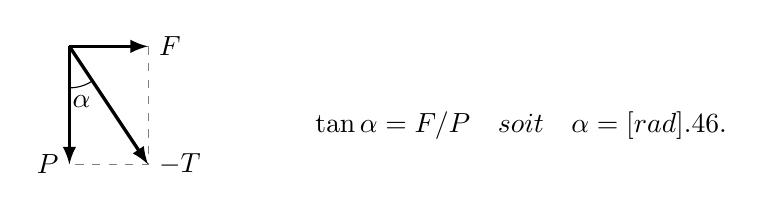
\begin{tikzpicture}[
		    force/.style={->,>=latex,draw=\JRLblue,very thick,nodes={\JRLblue}},
			]
			\draw[force](0,0)--(1,0)node[right]{$\vv{F}$};
			\draw[force](0,0)--(0,-1.5)node[left]{$\vv{P}$};
			\draw[force](0,0)--(1,-1.5)node[right]{$-\vv{T}$};
			\draw[gray,dashed](1,0)|-(0,-1.5);
			\draw (-56.3:15pt)arc(-56.3:-90:15pt);
			\draw (-73:15pt)node[below]{$\alpha$};
			\draw (3,-1)node[right]{$\tan\alpha=F/P
			\quad\text{soit}\quad\alpha=\np[rad]{.46}$.};
		\end{tikzpicture}
	\end{center}
	On peut aussi utiliser les produits scalaires. Par exemple,
	\[
		\vv{T}\cdot \vv{F}=T\times F\cos(\pi/2+\alpha)=-TF\sin\alpha.
	\]
	De plus, compte tenu de l'équilibre des forces, on a 
	\[
		\vv{T}\cdot \vv{F}=
		(-\vv{F}-\vv{P})\cdot \vv{F}=
		-F^2-\vv{P}\cdot \vv{F}=-F^2.
	\]
	Il en découle $\sin\alpha=F/T$ soit $\alpha=\np[rad]{.46}$ (c'est-à-dire $\alpha=\ang{26}$).
\end{corrige}

% ************************************** %

% =============================================================================== %
\finEntrainement
% =============================================================================== %










% ********************************************************************* %
%                           ENTRAÎNEMENT                                % 
% ********************************************************************* %
% ================ Métadonnées sur l'entraînement ===================== %
\titreEntrainementFacultatif	{Masse suspendue}
\hauteurLargeurCadreReponse		{6mm}{3cm}
\dureeResolutionFacultative		{3} % 1, 2, 3 ou 4
\typeEntrainement				{} % Newton ou QCM ou AN ou vide (exercice "normal")
\nombreColonnesQuestions		{1} % vide, 1, 2, 3, etc.
\avecPlusieursQuestions			{Y} % Y ou N
\initialisationEntrainement
% ===================================================================== %


% mmmmmmmmmmmmmmmmmmmmmmmmmmmmmmmmmmmmmmmmmmmmmmmmmmmmmmmmm %
% 		  Insertion d'une image en regard d'un texte
% mmmmmmmmmmmmmmmmmmmmmmmmmmmmmmmmmmmmmmmmmmmmmmmmmmmmmmmmm %
% --------------------------------------------------------- %
\pourcentageDeLaPartieAGauche   {0.5}
% --------------------------------------------------------- %
%                                                           %
% -------------------- Partie à gauche -------------------- %
%                                                           %
                                \initialisationPartieGauche % 
%                                                           %
%                                                           %
Un objet qui pèse \np[N]{800} est suspendu en équilibre à l'aide de deux cordes symétriques qui font un angle $\theta=\ang{20}$ avec la direction horizontale. 

Le point \ptA est soumis à trois forces : 
\[
\vv{T}, \vv{T'}\text{ et }\vv{F}.
\] 

On note $\vv{R}$ la résultante des forces.
% --------------------------------------------------------- %
%                                                           %
% -------------------- Partie à droite -------------------- %
%                                                           %
                                \initialisationPartieDroite %
%                                                           %
%                                                           %
\begin{center}
\subimport{_images/}{fiche_MCA02_masse_suspendue_JRL_v3.tex}
\end{center}
% --------------------------------------------------------- %
                               \finalisationDuPartageDePage %					
% --------------------------------------------------------- %



% =============================================================================== %
\debutEntrainement
% =============================================================================== %


% ^^^^^^^^^^^^^^^^^^^^^^^^^^^^^^^^^^^^^^ %
%               Question                 %
% ^^^^^^^^^^^^^^^^^^^^^^^^^^^^^^^^^^^^^^ %
\begin{enonce}
	 Exprimer la composante horizontale $R_x$ en fonction de $T$, $T'$ et $\theta$.
\end{enonce}

\reponse{$(T'-T)\cos\theta$}

\begin{corrige}
	On a $\vv{R}=\vv{T}+\vv{T'}+\vv{F}$. La composante horizontale de $\vv{R}$ vaut 
	\[
		R_x=\vv{R}\cdot \vv{e_x}=
		\underbrace{\vv{T}\cdot \vv{e_x}}_{-T\cos\theta}+
		\underbrace{\vv{T'}\cdot \vv{e_x}}_{T'\cos\theta}+
		\underbrace{\vv{F}\cdot \vv{e_x}}_{0}
		=(T'-T)\cos\theta.
	\]
\end{corrige}

% ************************************** %



% ^^^^^^^^^^^^^^^^^^^^^^^^^^^^^^^^^^^^^^ %
%               Question                 %
% ^^^^^^^^^^^^^^^^^^^^^^^^^^^^^^^^^^^^^^ %
\begin{enonce}
	 Exprimer la composante verticale $R_y$ en fonction de $T$, $T'$, $F$ et $\theta$.
\end{enonce}

\reponse{$(T'+T)\sin\theta-F$}

\begin{corrige}
	La composante verticale de $\vv{R}$ s'écrit 
	\[
		R_y=\vv{R}\cdot \vv{e_y}=
		\underbrace{\vv{T}\cdot \vv{e_y}}_{T\sin\theta}+
		\underbrace{\vv{T'}\cdot \vv{e_y}}_{T'\sin\theta}+
		\underbrace{\vv{F}\cdot \vv{e_y}}_{-F}
		=(T'+T)\sin\theta-F.
	\]
\end{corrige}

% ************************************** %




% ^^^^^^^^^^^^^^^^^^^^^^^^^^^^^^^^^^^^^^ %
%               Question                 %
% ^^^^^^^^^^^^^^^^^^^^^^^^^^^^^^^^^^^^^^ %
\begin{enonce}
Déterminer la tension $T$ en résolvant l'équation $\vv{R}=\vv{0}$.
\end{enonce}

\reponse{$\np[kN]{1.17}$}

\begin{corrige}
	Résoudre l'équation vectorielle $\vv{R}=\vv{0}$, c'est résoudre le système d'équations suivant :
	\[
		\left\{\begin{array}{rcl}
			(T'-T)\cos\theta	&=& 0\\
			(T'+T)\sin\theta-F	&=& 0
		\end{array}	\right.
		\quad\text{soit}\quad
		\left\{\begin{array}{rcl}
			T'	&=& T\\
			T	&=& \frac{F}{2\sin\theta}.
		\end{array}	\right.
	\]
	Sachant que $F=\np[N]{800}$ et $\theta=\ang{20}$, on obtient $T=\np[kN]{1.17}$.
\end{corrige}

% ************************************** %

% =============================================================================== %
\finEntrainement
% =============================================================================== %






% •••••••••••••••••••••••••••••••••••••••••••••••••••••••••••••••••••••••••••• %
\sectionFicheEntrainement{Mouvements rectilignes}
% •••••••••••••••••••••••••••••••••••••••••••••••••••••••••••••••••••••••••••• %




% ********************************************************************* %
%                           ENTRAÎNEMENT                                % 
% ********************************************************************* %
% ================ Métadonnées sur l'entraînement ===================== %
\titreEntrainementFacultatif	{Chute avec frottement}
\hauteurLargeurCadreReponse		{6mm}{3cm}
\dureeResolutionFacultative		{1} % 1, 2, 3 ou 4
\typeEntrainement				{AN} % Newton ou QCM ou AN ou vide (exercice "normal")
\nombreColonnesQuestions		{1} % vide, 1, 2, 3, etc.
\avecPlusieursQuestions			{N} % Y ou N
\initialisationEntrainement
% ===================================================================== %

Un corps de masse $m=\SI{2}{kg}$ tombe verticalement avec une accélération de $a= \SI{9}{m.s^{-2}}$. Lors de sa chute il subit la force de pesanteur ainsi qu'une force de frottement due à l'air.

On prendra $g=\SI{9,8}{m.s^{-2}}$ pour l'intensité du champ de pesanteur.

% =============================================================================== %
\debutEntrainement
% =============================================================================== %

% ^^^^^^^^^^^^^^^^^^^^^^^^^^^^^^^^^^^^^^ %
%               Question                 %
% ^^^^^^^^^^^^^^^^^^^^^^^^^^^^^^^^^^^^^^ %

\begin{enonce}
Combien vaut l'intensité de la force de frottement ?	 
\end{enonce}

\reponse{$\np[N]{1.6}$}

\begin{corrige}
	Le principe fondamental de la dynamique impose $m\vv{g}+\vv{F}=m \vv{a}$. En projetant la relation précédente suivant la verticale descendante, on obtient $mg-F=ma$ ce qui donne $F=m(g-a)=\np[N]{1.6}$. 
\end{corrige}

% ************************************** %

% =============================================================================== %
\finEntrainement
% =============================================================================== %




\newpage


% ********************************************************************* %
%                           ENTRAÎNEMENT                                % 
% ********************************************************************* %
% ================ Métadonnées sur l'entraînement ===================== %
\titreEntrainementFacultatif	{Contact dans un ascenseur}
\hauteurLargeurCadreReponse		{6mm}{3cm}
\dureeResolutionFacultative		{1} % 1, 2, 3 ou 4
\typeEntrainement				{AN} % Newton ou QCM ou AN ou vide (exercice "normal")
\nombreColonnesQuestions		{1} % vide, 1, 2, 3, etc.
\avecPlusieursQuestions			{N} % Y ou N
\initialisationEntrainement
% ===================================================================== %

Un homme de masse $m=\np[kg]{80}$ est dans un ascenseur qui monte avec une accélération $a = \SI{1}{m.s^{-2}}$. On note $\vv{F}$ la force exercée par l'homme sur le plancher de l'ascenseur.

On prendra $g=\SI{9,8}{m.s^{-2}}$ pour l'intensité du champ de pesanteur.

% =============================================================================== %
\debutEntrainement
% =============================================================================== %

% ^^^^^^^^^^^^^^^^^^^^^^^^^^^^^^^^^^^^^^ %
%               Question                 %
% ^^^^^^^^^^^^^^^^^^^^^^^^^^^^^^^^^^^^^^ %

\begin{enonce}
	 Combien vaut l'intensité de $\vv{F}$ ?
\end{enonce}

\reponse{$\np[N]{864}$}

\begin{corrige}
L'homme subit son poids $\vv{P}=m \vv{g}$ et la force de contact dû à l'ascenseur $-\vv{F}$ (principe des actions réciproques). Le principe fondamental de la dynamique donne $m\vv{g}-\vv{F}=m \vv{a}$. En projetant sur la verticale ascendante, on obtient 
$ma=-mg+F$, soit $F=m(a+g)=\SI{80}{kg}\times \SI{10,8}{m.s^{-2}}=\np[N]{864}$.
\end{corrige}

% ************************************** %
% =============================================================================== %
\finEntrainement
% =============================================================================== %








% ********************************************************************* %
%                           ENTRAÎNEMENT                                % 
% ********************************************************************* %
% ================ Métadonnées sur l'entraînement ===================== %
\titreEntrainementFacultatif	{Calcul d'une action de contact}
\hauteurLargeurCadreReponse		{7mm}{5cm}
\dureeResolutionFacultative		{2} % 1, 2, 3 ou 4
\typeEntrainement				{} % Newton ou QCM ou AN ou vide (exercice "normal")
\nombreColonnesQuestions		{1} % vide, 1, 2, 3, etc.
\avecPlusieursQuestions			{Y} % Y ou N
\initialisationEntrainement
% ===================================================================== %


%% mmmmmmmmmmmmmmmmmmmmmmmmmmmmmmmmmmmmmmmmmmmmmmmmmmmmmmmmm %
%% 		  Insertion d'une image en regard d'un texte
%% mmmmmmmmmmmmmmmmmmmmmmmmmmmmmmmmmmmmmmmmmmmmmmmmmmmmmmmmm %
%% --------------------------------------------------------- %
%\pourcentageDeLaPartieAGauche   {0.6}
%% --------------------------------------------------------- %
%%                                                           %
%% -------------------- Partie à gauche -------------------- %
%%                                                           %
%                                \initialisationPartieGauche % 
%%                                                           %
%%                                                           %
Un bloc de masse $m$, de poids $\vv{P}$ glisse à une vitesse $v(t)$, variable au cours du temps, sur un support plan qui exerce une action de contact. 

Celle-ci se décompose en deux actions : 
\begin{itemize}
	\item une action normale à la surface $\vv{f_\text{n}}$;
	\item une action de frottement $\vv{f_\text{t}}$ opposée à la vitesse de glissement.
\end{itemize}

Le plan est incliné d'un angle $\alpha$, comme figuré ci-dessous.
%% --------------------------------------------------------- %
%%                                                           %
%% -------------------- Partie à droite -------------------- %
%%                                                           %
%                                \initialisationPartieDroite %
%%                                                           %
%%                                                           %
\begin{center}
\subimport{_images/}{fiche_MCA02_frottement_incline_JRL_v3.tex}
\end{center}
%% --------------------------------------------------------- %
%                               \finalisationDuPartageDePage %					
%% --------------------------------------------------------- %


Déterminer (en fonction d'au moins une des données $P$, $v(t)$, $m$ et $\alpha$) :


% =============================================================================== %
\debutEntrainement
% =============================================================================== %

% ^^^^^^^^^^^^^^^^^^^^^^^^^^^^^^^^^^^^^^ %
%               Question                 %
% ^^^^^^^^^^^^^^^^^^^^^^^^^^^^^^^^^^^^^^ %
\begin{enonce}
l'intensité de l'action normale $f_\text{n}$
\end{enonce}

\reponse{$P\cos\alpha$}

\begin{corrige}
Le principe fondamental de la dynamique donne $\vv{P}+\vv{f_\text{n}}+\vv{f_\text{t}}=m \vv{a}$ avec $\vv{a}=\diff{v}{t}\,\vv{e_\text{t}}$ ($\vv{e_\text{t}}$ est le vecteur unitaire orienté suivant le vecteur vitesse ; c'est le vecteur tangent de la base de Frenet). Si l'on projette la relation suivant la normale $\vv{e_\text{n}}$ au support on aboutit à 
	\[
		\underbrace{\vv{P}\cdot \vv{e_\text{n}}}_{P\cos(\pi-\alpha)}+
		\underbrace{\vv{f_\text{n}}\cdot \vv{e_\text{n}}}_{f_\text{n}}+
		\underbrace{\vv{f_\text{t}}\cdot \vv{e_\text{n}}}_{0}=
		m \frac{\mathrm{d}v}{\mathrm{d} t}\, \underbrace{\vv{e_\text{t}}\cdot \vv{e_\text{n}}}_{0},
	\]
	ce qui donne $f_\text{n}=-P\cos(\pi-\alpha)=P\cos\alpha$.
\end{corrige}
% ************************************** %

% ^^^^^^^^^^^^^^^^^^^^^^^^^^^^^^^^^^^^^^ %
%               Question                 %
% ^^^^^^^^^^^^^^^^^^^^^^^^^^^^^^^^^^^^^^ %
\begin{enonce}
l'intensité du frottement $f_\text{t}$
\end{enonce}

\reponse{$-m \frac{\mathrm{d}v}{\mathrm{d} t}+P\sin\alpha$}

\begin{corrige}
En projetant la relation fondamentale de la dynamique suivant la direction tangentielle au support, on obtient 
	\[
		\underbrace{\vv{P}\cdot \vv{e_\text{t}}}_{P\cos(\pi/2-\alpha)}+
		\underbrace{\vv{f_\text{n}}\cdot \vv{e_\text{t}}}_{0}+
		\underbrace{\vv{f_\text{t}}\cdot \vv{e_\text{t}}}_{-f_\text{t}}=
		m\frac{\mathrm{d}v}{\mathrm{d} t}\, \underbrace{\vv{e_\text{t}}\cdot \vv{e_\text{t}}}_{1},
	\]
	c'est-à-dire $f_\text{t}=-m \frac{\mathrm{d}v}{\mathrm{d} t}+P\sin\alpha$.
\end{corrige}
% ************************************** %

% =============================================================================== %
\finEntrainement
% =============================================================================== %





% ********************************************************************* %
%                           ENTRAÎNEMENT                                % 
% ********************************************************************* %
% ================ Métadonnées sur l'entraînement ===================== %
\titreEntrainementFacultatif	{Calcul d'une accélération}
\hauteurLargeurCadreReponse		{6mm}{3cm}
\dureeResolutionFacultative		{3} % 1, 2, 3 ou 4
\typeEntrainement				{} % Newton ou QCM ou AN ou vide (exercice "normal")
\nombreColonnesQuestions		{1} % vide, 1, 2, 3, etc.
\avecPlusieursQuestions			{Y} % Y ou N
\initialisationEntrainement
% ===================================================================== %


% mmmmmmmmmmmmmmmmmmmmmmmmmmmmmmmmmmmmmmmmmmmmmmmmmmmmmmmmm %
% 		  Insertion d'une image en regard d'un texte
% mmmmmmmmmmmmmmmmmmmmmmmmmmmmmmmmmmmmmmmmmmmmmmmmmmmmmmmmm %
% --------------------------------------------------------- %
\pourcentageDeLaPartieAGauche   {0.5}
% --------------------------------------------------------- %
%                                                           %
% -------------------- Partie à gauche -------------------- %
%                                                           %
                                \initialisationPartieGauche % 
%                                                           %
%                                                           %
Deux blocs $\ptB_1$ et $\ptB_2$ de masse respective $2m$ et $m$ sont reliés par un fil. %inextensible de masse négligeable.
On passe le fil dans la gorge d'une poulie, % de masse nulle fixée à une table, 
puis on maintient le bloc B$_{1}$ sur la table alors que l'autre est suspendu dans l'air. On libère le bloc B$_{1}$ qui glisse alors sur la table. On note $T_1$ et $T_2$ les tensions exercées par le fil sur les blocs, $a_1$ et $a_2$ les accélérations respectives des blocs $\ptB_1$ et $\ptB_2$, et $g$ le champ de pesanteur. 

Les frottements sont négligeables.
% --------------------------------------------------------- %
%                                                           %
% -------------------- Partie à droite -------------------- %
%                                                           %
                                \initialisationPartieDroite %
%                                                           %
%                                                           %
\begin{center}
\subimport{_images/}{fiche_MCA02_deux_masses_JRL_v3.tex}
\end{center}
% --------------------------------------------------------- %
                               \finalisationDuPartageDePage %					
% --------------------------------------------------------- %


% =============================================================================== %
\debutEntrainement
% =============================================================================== %


% ^^^^^^^^^^^^^^^^^^^^^^^^^^^^^^^^^^^^^^ %
%               Question                 %
% ^^^^^^^^^^^^^^^^^^^^^^^^^^^^^^^^^^^^^^ %

\begin{enonce}
	 Exprimer $a_1$ en fonction de $m$ et $T_1$. 
\end{enonce}

\reponse{$\frac{T_1}{2m}$}

\begin{corrige}
	Le principe fondamental appliqué au bloc $\text{B}_1$ donne $2m\vv{g}+\vv{R}+\vv{T_1}=2m \vv{a_1}$. En projetant cette relation suivant le sens du mouvement, on obtient : 
	\[
		2m\underbrace{\vv{g}\cdot\vv{e_x}}_{0}+
		\underbrace{\vv{R}\cdot\vv{e_x}}_{0}+
		\underbrace{\vv{T_1}\cdot\vv{e_x}}_{T_1}=
		2m \underbrace{\vv{a_1}\cdot\vv{e_x}}_{a_1}
		\quad\text{soit}\quad
		a_1=\frac{T_1}{2m}.
	\]
\end{corrige}

% ************************************** %


% ^^^^^^^^^^^^^^^^^^^^^^^^^^^^^^^^^^^^^^ %
%               Question                 %
% ^^^^^^^^^^^^^^^^^^^^^^^^^^^^^^^^^^^^^^ %

\begin{enonce}
	 Exprimer l'accélération $a_2$ de $\ptB_2$ en fonction de $m$, $g$ et $T_2$. 
\end{enonce}

\reponse{$g-\frac{T_2}{m}$}

\begin{corrige}
	Le principe fondamental appliqué au bloc $\ptB_2$ donne $m\vv{g}+\vv{T_2}=m \vv{a_2}$. En projetant cette relation suivant le sens du mouvement, on obtient : 
	\[
		m\underbrace{\vv{g}\cdot\vv{e_y}}_{g}+
		\underbrace{\vv{T_2}\cdot\vv{e_y}}_{-T_2}=
		m \underbrace{\vv{a_2}\cdot\vv{e_y}}_{a_2}
		\quad\text{soit}\quad
		a_2=g-\frac{T_2}{m}.
	\]
\end{corrige}

% ************************************** %


% =============================================================================== %
\pauseEntrainement
% =============================================================================== %

Le fil étant inextensible et sans masse on a $a_1=a_2$ et $T_1=T_2$.

% =============================================================================== %
\repriseEntrainement
% =============================================================================== %



% ^^^^^^^^^^^^^^^^^^^^^^^^^^^^^^^^^^^^^^ %
%               Question                 %
% ^^^^^^^^^^^^^^^^^^^^^^^^^^^^^^^^^^^^^^ %

\begin{enonce}
En déduire l'accélération en fonction uniquement de $g$
\end{enonce}

\reponse{$\frac{g}{3}$}

\begin{corrige}
	On a les relations : 
	\[
	a_1=\frac{T_1}{2m}
	\qquad\text{et}\qquad
	a_2=g-\frac{T_2}{m}.
	\]
	Multiplions la première relation par $2m$, et la deuxième par $m$, puis additionnons les. On trouve 
	\[
	2ma_1+ma_2=T_1+mg-T_2.
	\]
	 Comme $a_1=a_2$ et $T_1=T_2$, on obtient $3ma_1=mg$ soit $a_1=a_2=g/3$.
\end{corrige}

% ************************************** %


% =============================================================================== %
\finEntrainement
% =============================================================================== %






% ---------------------------------------------------------------------------- %
%                       Affichage des réponses mélangées                       %
% ---------------------------------------------------------------------------- %
\afficheReponsesMelangees
% ---------------------------------------------------------------------------- %

%%%%%%%%%%%%%%%%%%%%%%%%%%%%%%%%%%%%%%%%%%%%%%%%%%%%%%%%%%%%%%%%%%%%%%%%%%%%%%%%%%%%%%%%%%%%%%
\finFicheEntrainement                                                                        %
%%%%%%%%%%%%%%%%%%%%%%%%%%%%%%%%%%%%%%%%%%%%%%%%%%%%%%%%%%%%%%%%%%%%%%%%%%%%%%%%%%%%%%%%%%%%%%




% ======================================================= % 
% ============== Gestion de la compilation ============== %
% ======================================================= % 
\ifdefined\mainIsLoaded\else
\printReponsesEtCorriges
\end{document}\fi
% ======================================================= % 
% ======================================================= % 
